\documentclass[10pt, letterpaper]{article}
\usepackage[utf8]{inputenc}
\usepackage{amsmath}
\usepackage{amssymb}
\usepackage{bbm}
\usepackage{booktabs}
\usepackage{caption}
\usepackage{color}
\usepackage[shortlabels]{enumitem}
\usepackage{fancyhdr}
\usepackage{hyperref}
\usepackage{geometry}
\geometry{a4paper,scale=0.8}
\usepackage{graphicx}
\graphicspath{ {./img/}}
\usepackage{listings}
\usepackage{mathtools}
\usepackage{mathrsfs}
\usepackage{setspace}
\renewcommand{\baselinestretch}{1.3}

% set-up header & footer
\pagestyle{empty}
\fancyhf{}
\cfoot{\thepage}
\lhead{%
\textbf{University of California, Berkeley} \\
Department of Civil \& Environ. Eng.
}
\rhead{\textbf{CS 285 Deep Reinforcement Learning}\\\date{\today}}

\title{%
    \textbf{Homework 1}
}
\author{Juanwu Lu (3037432593)\\ \small(M.Sc. Civil Engineering, UC Berkeley)}
\date{}

% set-up code listing
\definecolor{dkgreen}{rgb}{0,0.6,0}
\definecolor{gray}{rgb}{0.5,0.5,0.5}
\definecolor{manuve}{rgb}{0.58,0,0.82}

\lstset{frame=tb,
    language=Python,
    aboveskip=3mm,
    belowskip=3mm,
    showstringspaces=false,
    columns=flexible,
    basicstyle={\small\ttfamily},
    numbers=none,
    numberstyle=\tiny\color{gray},
    keywordstyle=\color{blue},
    commentstyle=\color{dkgreen},
    stringstyle=\color{manuve},
    breaklines=true,
    breakatwhitespace=true,
    tabsize=3
}

\begin{document}
    \maketitle
    \captionsetup[figure]{labelfont={bf},labelformat={default},labelsep=period,name={Figure}}
    \captionsetup[table]{labelfont={bf},labelformat={default},labelsep=period,name={TABLE}}
    \thispagestyle{fancy}

    % Problem 1
    \section{Behavior Cloning}
    \subsection{Task report}
    \begin{table}[htbp]
        \centering
        \caption{Behavior Cloning (BC) Policy's Return over 30 rollouts. In both environments, the policy distribution mean network is an two-layer MLP with a hidden size of 64. The Ant-v4 and the HalfCheetah-v4 have action sizes of 8 and 6. The number of training iteration is one for both environments with a training batch size of 100. The \texttt{ep\_len} is 1000 and the \texttt{eval\_batch\_size} is 30000 for both tasks. The \texttt{seed} is 42.}
        \begin{tabular}{@{}lccc@{}}
            \toprule
            \multicolumn{1}{c}{\textbf{Environment}} & \multicolumn{1}{l}{\textbf{Expert Return}} & \textbf{Mean Return} & \textbf{Standard Return} \\ \midrule
            Ant-v4                                   & 4713.6533                                  & 1397.3680            & 1033.6208                \\
            HalfCheetah-v4                           & 4205.7783                                  & 2795.4690            & 112.1943                 \\ \bottomrule
            \end{tabular}
        \label{tab:1}
    \end{table}

    \subsection{Hyperparameter set}
    \begin{figure}[htbp]
        \centering
        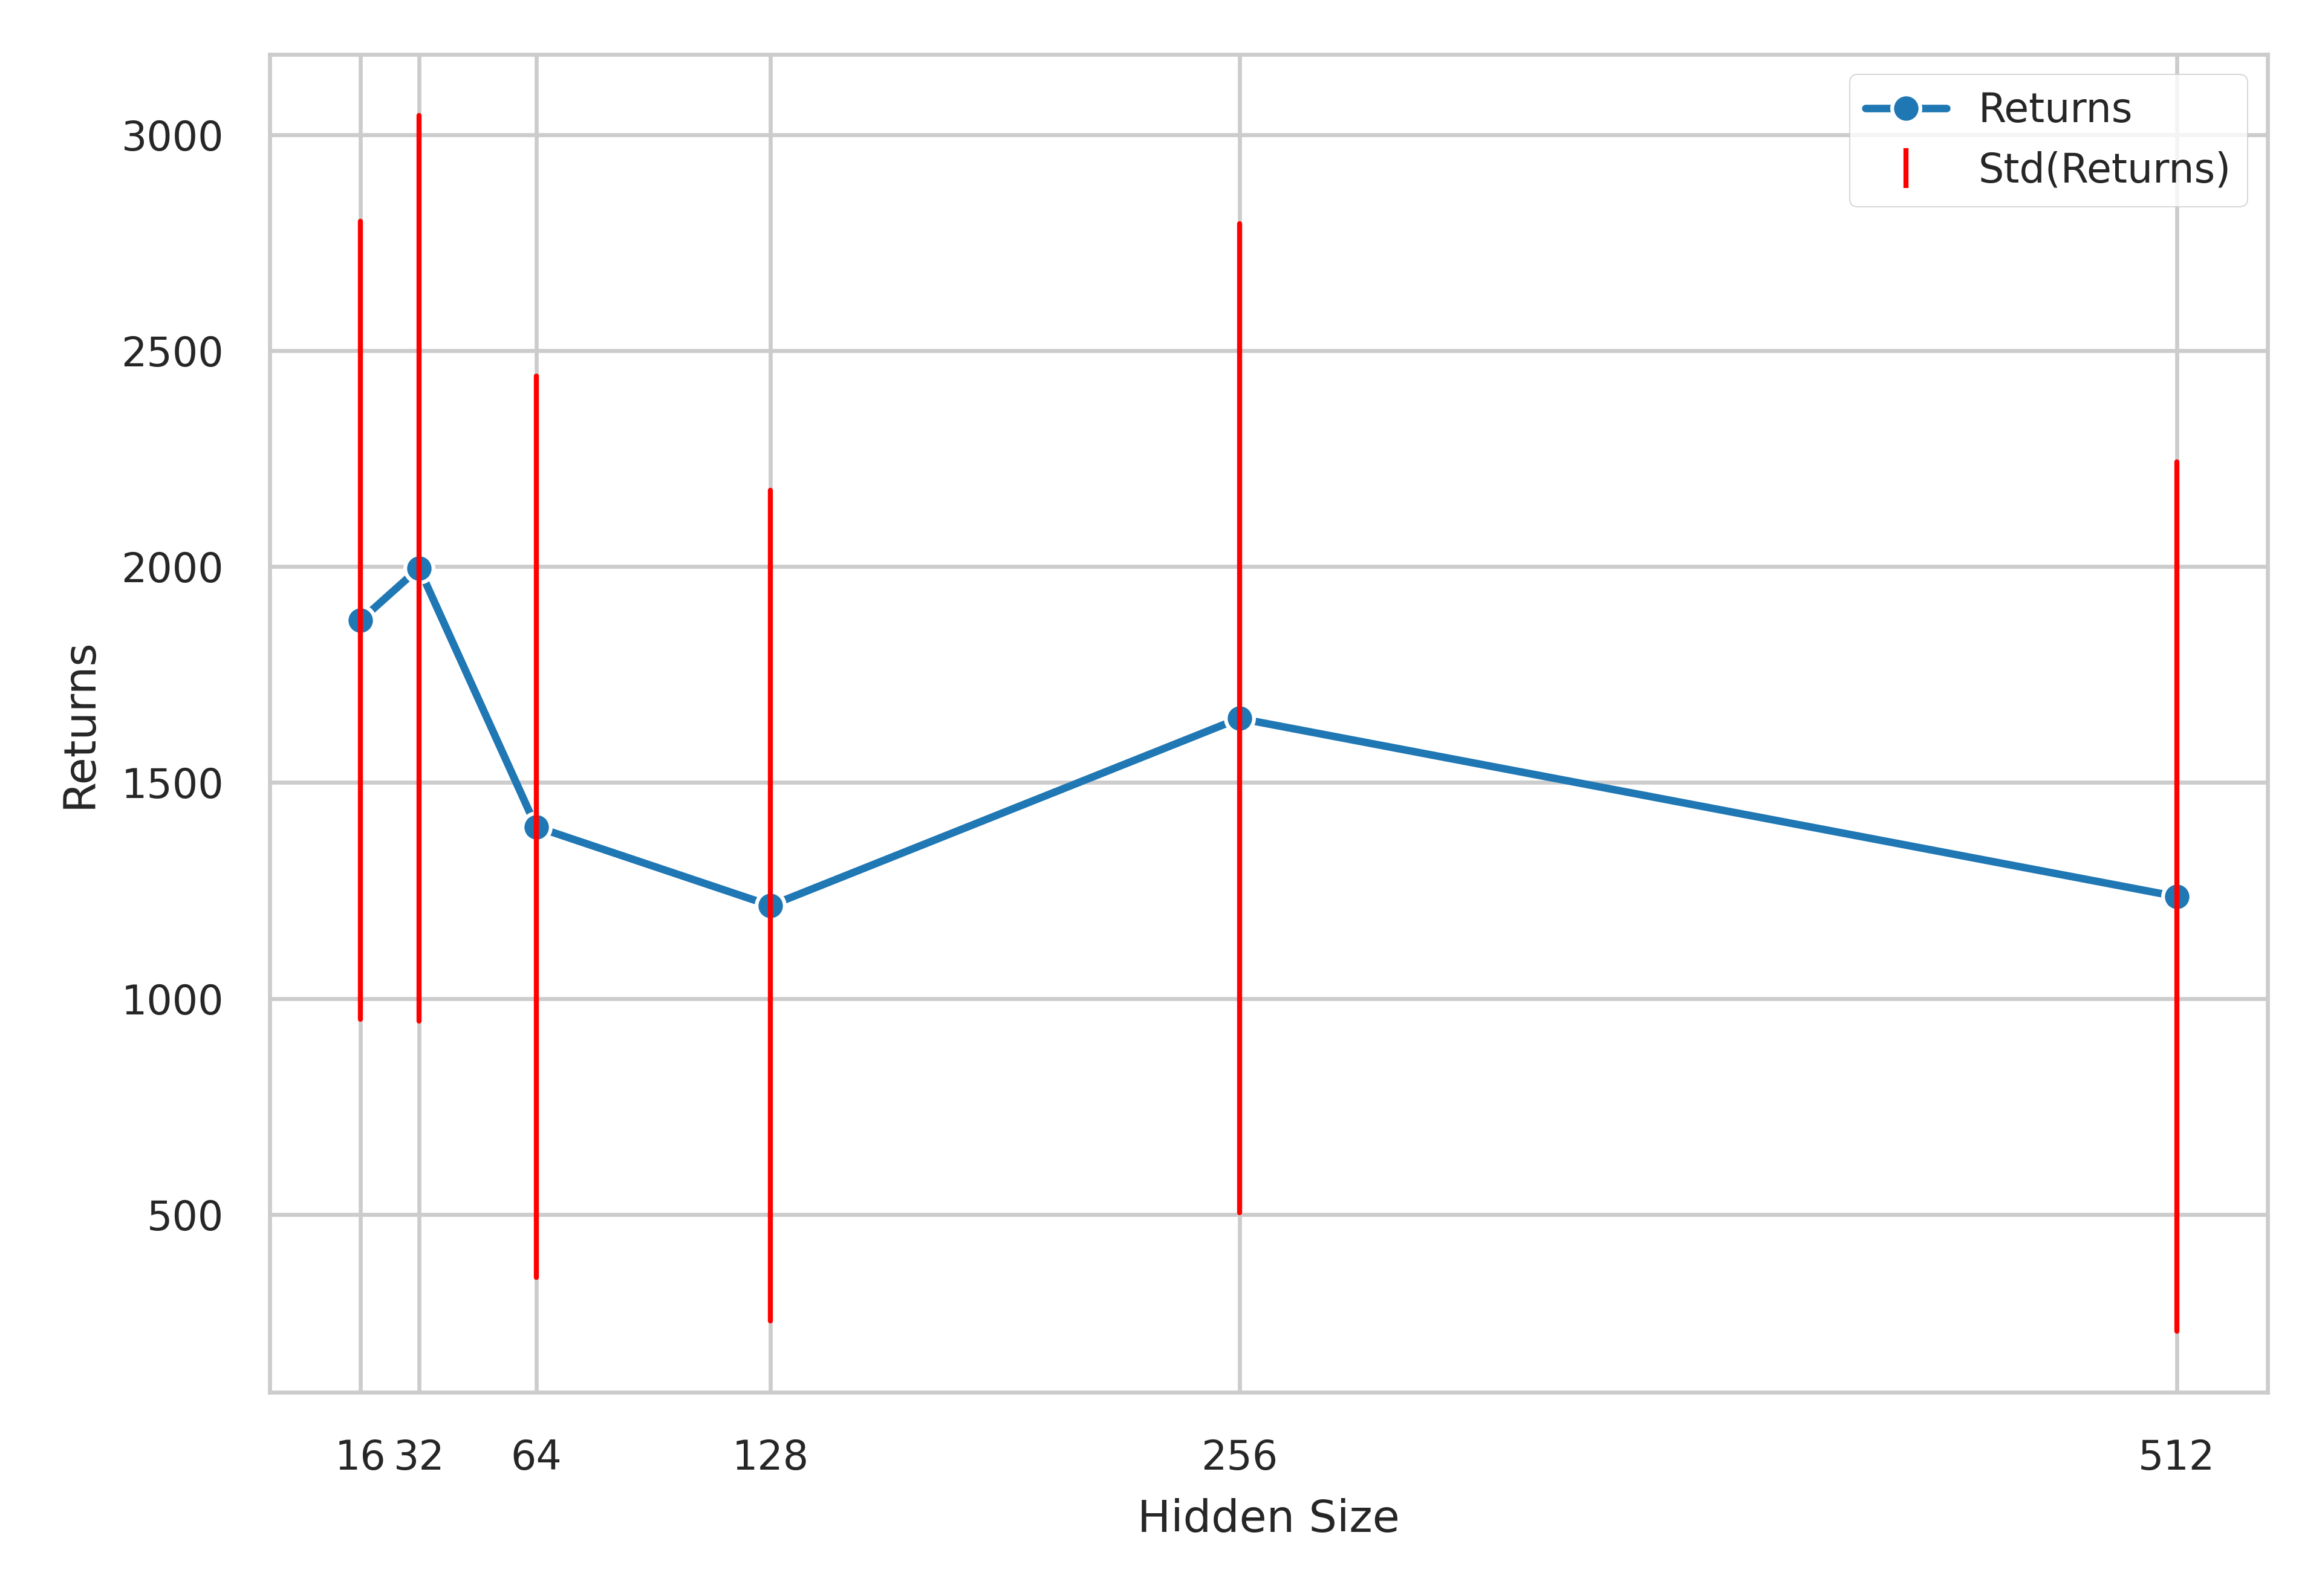
\includegraphics[width=0.7\textwidth]{img/q_1_3.png}
        \caption{Evaluation Returns vs. Sizes of Hidden Layers. With different settings of the hidden layer neurons, the neural network shows different capability of representing non-linear relationship between input observation features to output action probabilities. However, the performance is not plain linear increasing with respect to increasing hidden sizes since the complexity of the network trades off marginal performance increase with fixed training steps.}
        \label{fig:1}
    \end{figure}

    % Problem 2
    \section{DAgger}
    \begin{figure}[htbp]
        \centering
        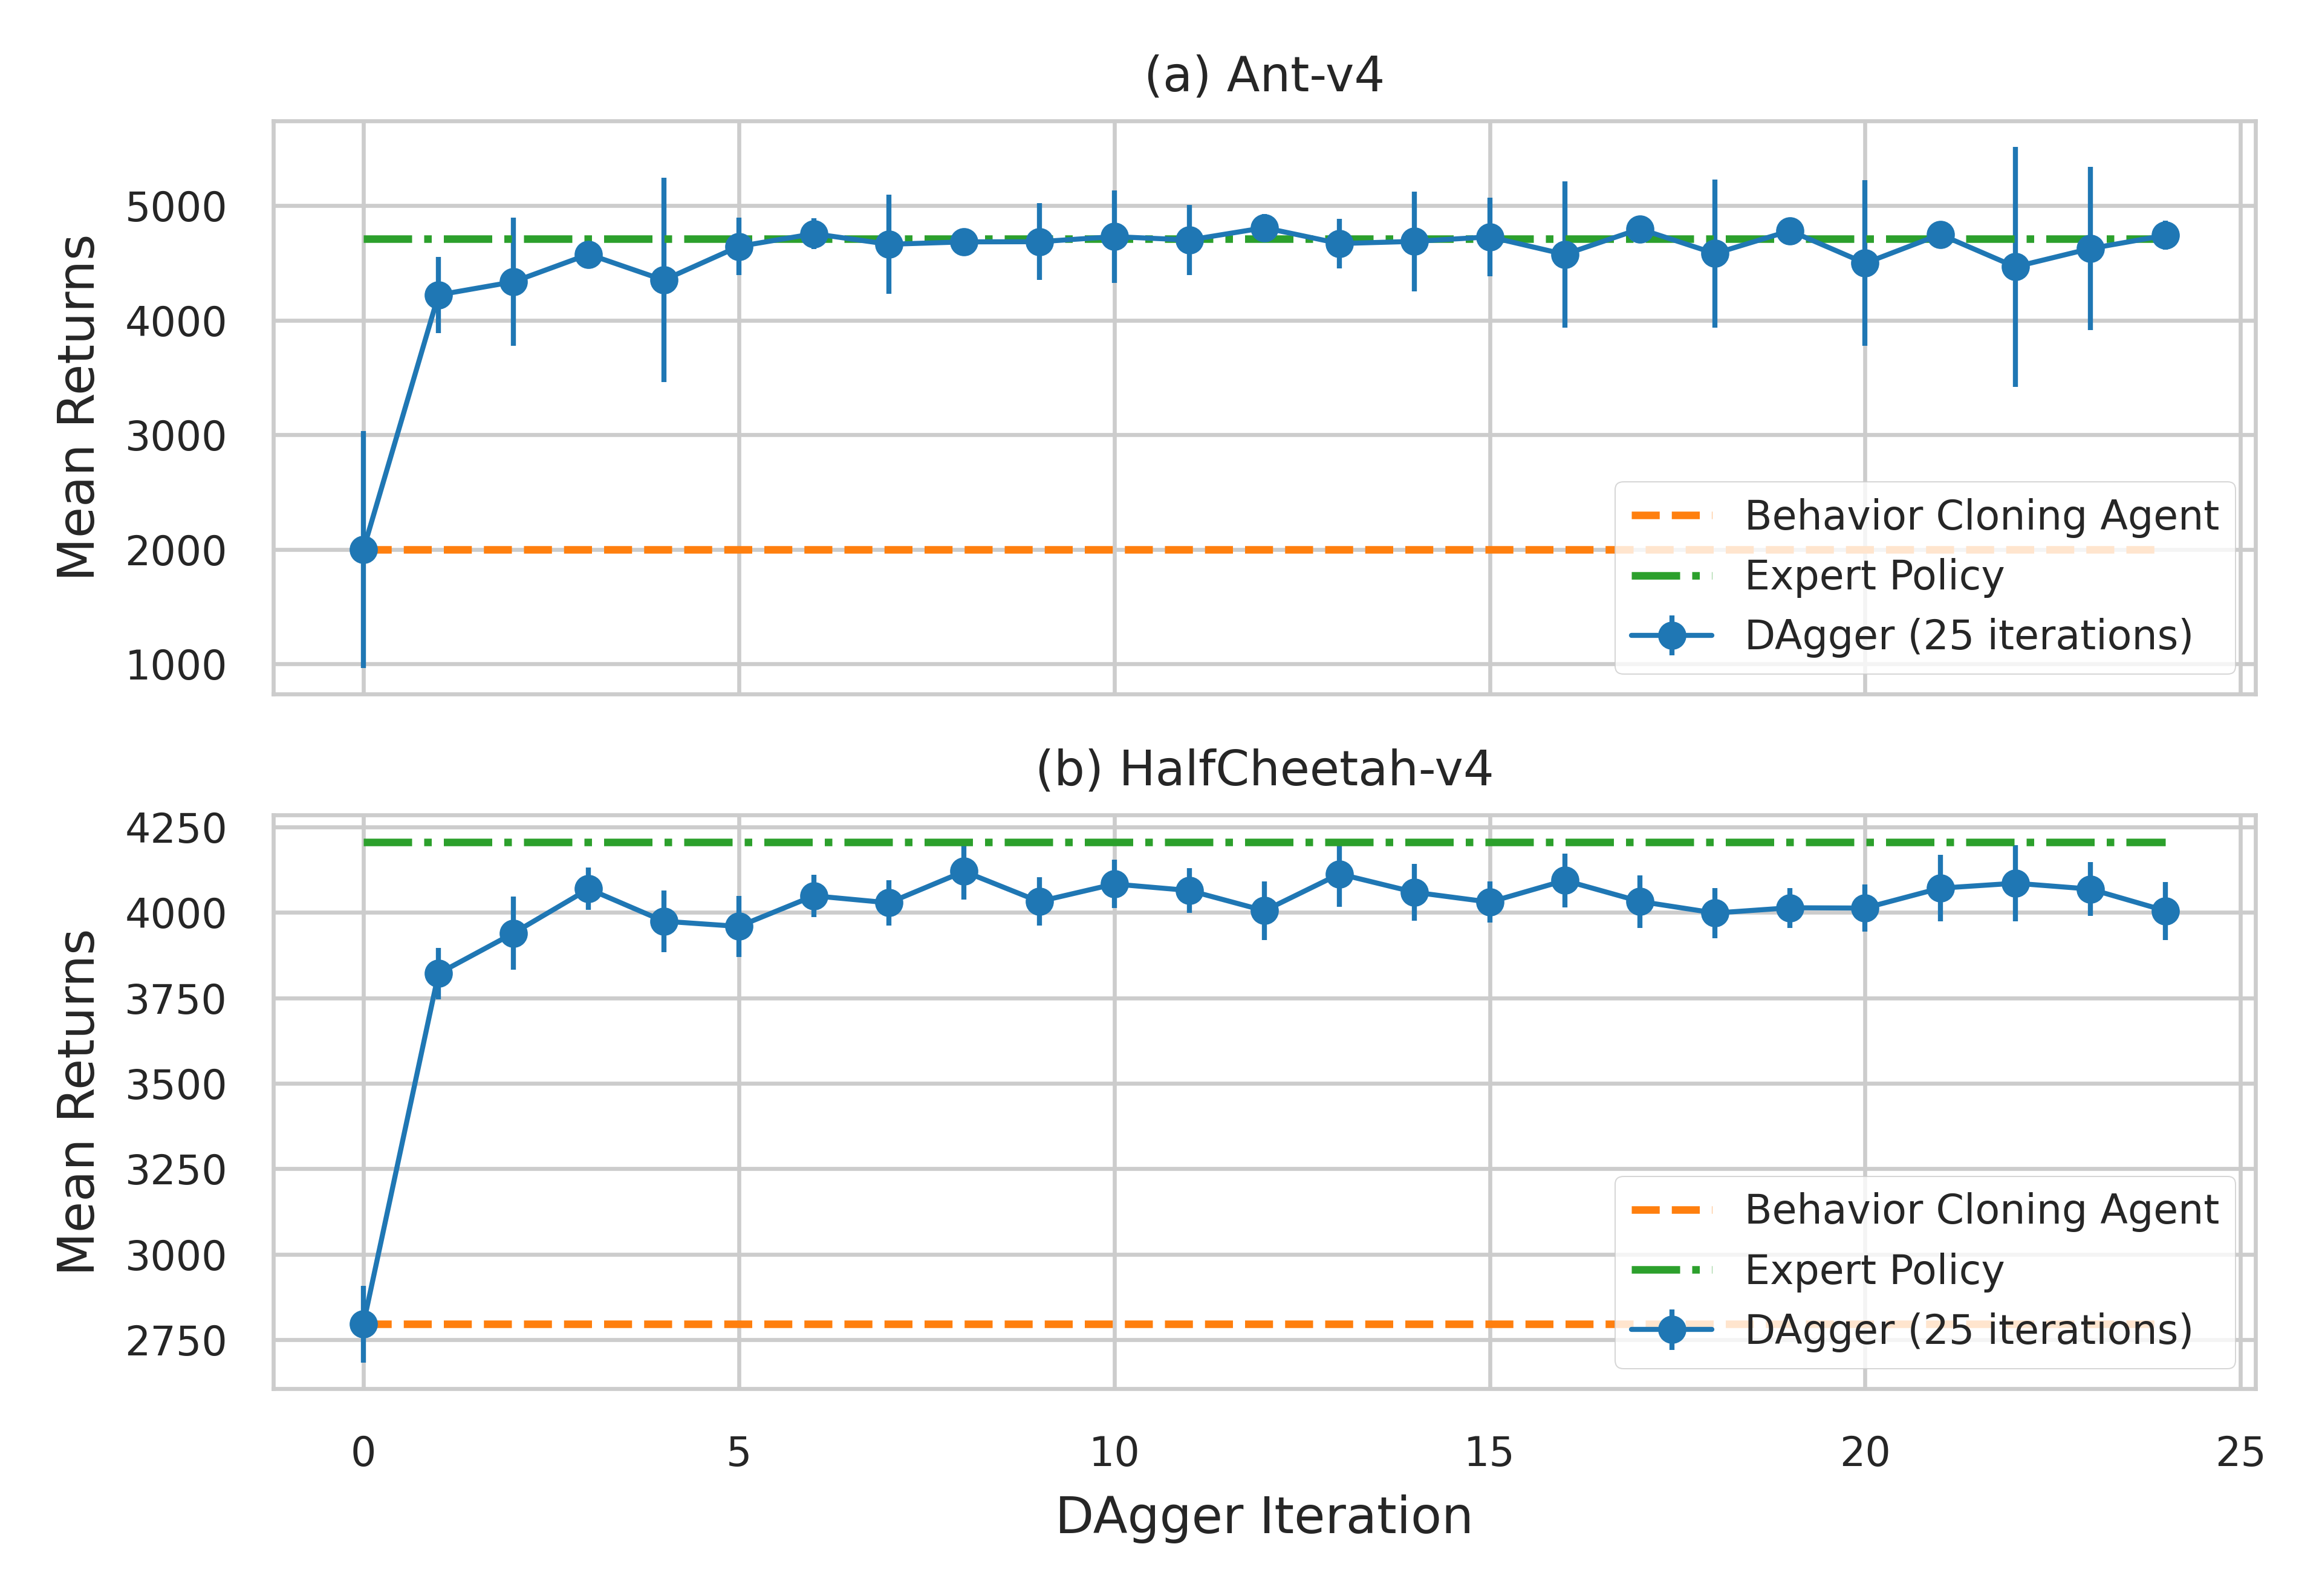
\includegraphics[]{img/q_2_2.png}
        \caption{(a) The Number of DAgger Iterations vs. the Policy's Mean Returns on the Ant-v4 Environment. Model is trained on a two-layer MLP with a hidden size of 32. The \texttt{train\_batch\_size}, \texttt{eval\_batch\_size}, and \texttt{ep\_len} are 100, 30000, and 1000, respectively. The \texttt{seed} is 42. (b) The Number of DAgger Iterations vs. the Policy's Mean Returns on the HalfCheetah-v4 Environment. Model is trained on a two-layer MLP with a hidden size of 64. The \texttt{train\_batch\_size}, \texttt{eval\_batch\_size}, and \texttt{ep\_len} are 100, 30000, and 1000, respectively. The \texttt{seed} is 42.}
        \label{fig:2}
    \end{figure}
    
\end{document}